\documentclass{article}

\usepackage{graphicx}
\usepackage{hyperref}
\usepackage[a4paper, margin=1.25in]{geometry}
\usepackage{breakcites}
\usepackage{subcaption}
\usepackage{float}
\usepackage{textcomp}
\usepackage{amsmath}
\usepackage{textgreek}
\usepackage{authblk}
\usepackage{rotating}
\usepackage{booktabs}
\usepackage{longtable}
\usepackage{pdflscape}
\usepackage{lineno}
\usepackage[
  style=numeric,
  citestyle=numeric-comp,
  backend=biber,
  doi=true,
  natbib=true,
  sorting=none
]{biblatex}

\addbibresource{library.bib}

\begin{document}

\title{Monitoring and Projecting Global Hunger}

\author[1,2,*]{Matthew Cooper}
\author[2,3]{Benjamin Müller}
\author[4]{Carlo Cafiero}
\author[2,5]{Juan Carlos Laso Bayas}
\author[5,6]{Jesús Crespo Cuaresma}
\author[2,7]{Homi Kharas}

\affil[1]{T.H. Chan School of Public Health, Harvard University}
\affil[2]{The World Data Lab, Vienna, Austria}
\affil[3]{Department of Economics, Vienna University of Economics and Business}
\affil[4]{The Food and Agricultural Organization of the United Nations}
\affil[5]{The International Institute for Applied Systems Analysis}
\affil[6]{Wittgenstein Centre For Demography and Global Human Capital}
\affil[7]{The Brookings Institute}
\affil[*]{Corresponding Author: mcooper@hsph.harvard.edu}

\maketitle
\begin{abstract}
Using microdata from 75 countries collected by the FAO and Gallup World Poll for the Voices of the Hungry project, we modeled levels of food security at the subnational level from 2010 to 2030 to create the \href{https://worldhunger.io}{World Hunger Clock}.  This is the first global picture at a subnational level of the Food Insecurity Experience Scale, the food security metric most indicative of the lived experience of hunger.  We find significant heterogeneity in food security around the world, ranging from less than 4\% of the population food insecure in some high-income countries to the parts of developing world where over half the population is severely food insecure.  Examining global temporal trends and accounting for the effects of the COVID-19 pandemic, we find that rates of food insecurity have been steadily declining, with large observed and forecasted gains in lower and lower-middle income countries, and decreases in total number of severely food insecure people.  However, the total number of moderately food insecure people has been increasing and, after recovering from the shock of the COVID-19 pandemic, will continue to increase through the end of the 2020s.  Overall, we conclude that global gains have been incremental, and current trends in development and demographic change will still leave a large share of the world's population experiencing hunger by 2030.  \end{abstract}

\section{Main}
Food security is a critical component of human flourishing and its importance as a global policy objective is reflected in the second Sustainable Development Goal (SDG 2), ``Zero Hunger." One of the indicators to track progress on the first target of this goal, to ensure access by everyone to safe, nutritious and sufficient food (SDG2.1), is the prevalence of at least moderate food insecurity in the population based on the Food Insecurity Experience Scale, or FIES. The FIES was developed by FAO in 2013 as a global extension of pioneering work done on Latin America to develop a metric of food insecurity based on the perspective of people who experience hunger and conditions that produce hunger. Other indicators of food insecurity, such as FAO's most commonly used estimate of undernourishment, are based on macro models of the mean and distribution of calories available per capita in a population. These do not directly capture the actual lived exposure of individuals to food shortages. 

The FIES is based on responses to polls and the data are limited to 75 countries where these have been conducted and microdata has been vetted and released by the FAO. The current practice is to assign the average regional prevalence rate for countries without survey data in order to compile regional and global aggregates. In addition, since the FIES is a relatively new metric, it does not have a sufficiently long time series to assess time trends with a reasonable degree of precision. To understand whether SDG 2 is being met, estimates of food insecurity outcomes in 2030 are required.

This paper contributes to shifting the research frontier by filling these two gaps in terms of data coverage and forecasts by developing a statistical model of FIES outcomes based on covariates that are available for territories where actual polling data are not available. Such a model can be employed to obtain forecasts to 2030 and assess likely future trends in food insecurity. We take advantage of individual-level characteristics collected in FIES surveys to push the analysis beyond the country level to a sub-national level. To our knowledge, this is the first effort to model the FIES outcomes at that scale.

Food security has traditionally been difficult to measure, and this has led to an incomplete or inaccurate assessment of global hunger. Metrics of macro-health, such as anthropometric measures and mortality rates are correlated broadly with food insecurity and have been used for many years to monitor human well-being \citep{Puffer1973, Habicht1974}.  However, these metrics are affected by other determinants of health such as the occurrence of infectious diseases, and are not meaningful at the scale of individuals or households \citep{Perumal2018}.  Other proxies for food security, such as food availability estimated from crop yields \citep{Maxwell1992}, are also inadequate because they only make rough estimates of how accessible food is to the general population, and can elide populations that are food insecure due to poor access, even when aggregate food availability is high \citep{Sen1983}.  Moreover, these metrics are very sensitive to incorrect estimates of crop yields and food reserves at a national scale.  Thus, global estimates of hunger and food insecurity based on these metrics carry forward similar flaws.

As researchers began to focus on food insecurity at the individual and household level, household microdata collecting information on household finances and consumption became a common proxy for food security \citep{Haddad1994}.  However, these efforts were criticized for being onerous, insufficiently comparable, as well as for ignoring subjective and experiential aspects of food security \citep{Maxwell1996}.  This led to the emergence of several indicators designed to be rapidly deployable, and based on the lived experience of food security \citep{Jones2013}.  These metrics include the Household Food Security Survey Module (HFSSM) \citep{kennedy2005keynote}, originally developed for use in the US; the Latin American and Caribbean Food Security Scale (ELCSA); and the Household Food Insecurity and Access Scale (HFIAS) \citep{Coates2007}.

Drawing on the insights derived in designing and implementing these novel food security metrics, the FIES was developed by the Food and Agricultural Organization (FAO) of the UN \cite{Ballard2013} and is now recognized as a rapidly deployable and cross-culturally valid tool for understanding individual and household-level food insecurity \citep{wambogo2018validity, smith2017world}.  The FIES is based on a survey of eight behaviors indicative of food insecurity and hunger over the previous year, such as skipping meals or worrying about having enough to eat.  Using a Rasch model \citep{Cafiero2018}, each individual in the survey is given a severity score that maximizes the likelihood of observing the responses given to the 8 questions asked in the survey.  Once individuals are ranked in this fashion, thresholds for moderate and severe food insecurity are set that describe people's experiences, and the prevalence of such food insecurity events can be computed. A moderately food insecure adult is likely to have compromised on food quality and variety as a result of lack of income, has been unsure about their ability to obtain food and has skipped meals or run out of food occasionally. A severely food insecure adult is likely to have run out of food and has gone an entire day without eating at times during the year.  Because the model estimates the population over a threshold on a univariate food insecurity scale, the percentage of people over the threshold for moderate food insecurity includes people that are also over the threshold for severe food insecurity.

Since 2014, in partnership with Gallup World Poll, the FAO administered the FIES in surveys around the world. The FAO uses this data to estimate the prevalence of food insecurity, and reports national-level estimates of the percentage of the population over the thresholds for moderate and severe food insecurity.  Drawing on individual-level data from these microdatasets in 75 countries, we use machine learning methods to estimate levels of food insecurity globally at the subnational level.  The model is then used to forecast food insecurity to the year 2030 under a middle-of-the-road scenario.

\section{Results}
\subsection{Food Insecurity over Time}
Globally, in the year 2020, we estimate that 820 million people are above the threshold for severe food insecurity, and 2.5 billion people are above the threshold for moderate food insecurity (See Fig. \ref{fig:timeseries}). These numbers are higher than the estimates in the 2020 FAO State of Food Insecurity report, which reports about 746 million severely food insecure people and 2 billion people experiencing at least moderate food insecurity in 2019 \citep{sofi2020}. 

Under realistic scenario assumptions, we find divergent trends in the number of moderate and severely food insecure people around the world, with the number of people at least moderately food insecure increasing and the number of people severely food insecure declining.  However, for both indicators, these changes are very slight: in 2030, the number of moderately food insecure people will have increased by 2.2\% since 2010, and the number of severely food insecure people will have decreased by 7.0\%.  The increases in moderate food insecurity have been in lower and lower-middle income countries, while the increases in severe food insecurity are entirely from lower income countries.  For both the moderate and severe food insecurity thresholds, COVID-19 has had a clearly discernible impact, particularly in middle-income countries.

\begin{figure}[H]
  \centering
  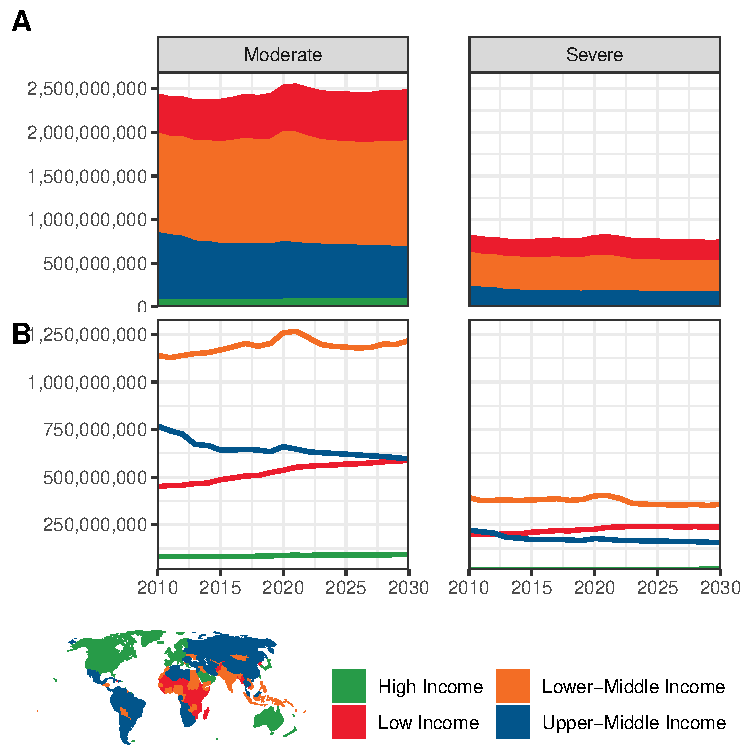
\includegraphics[width=\linewidth]{img/TimeSeries.pdf}
  \caption{Number of people over the thresholds for moderate and severe food insecurity, by World Bank income groups as of 2020.  Panel (A) shows the number of food insecure people with region totals stacked, to show global trends and totals over time.  Panel (B) shows regional totals compared against each other over time.}
  \label{fig:timeseries}
\end{figure}

Examining the rate of food insecurity in a population, rather than the total number of food insecure people (See Fig. \ref{fig:rates}, we find clear improvements in all except high income countries.  Countries that are currently upper-middle income, like China and Brazil, saw large gains in improving food insecurity rates throughout the 2010s, and will continue to see somewhat diminished gains in improving food security throughout the 2030s.  Lower and lower-middle income countries, on the other hand, saw more modest gains in the 2010s but are forecasted to see greater gains in reducing the rate of food insecurity in 2020s.  In spite of this progress in the bottom three income quartiles, in high-income countries, the rates of people in moderate and severe food insecurity have been flat and are expected even to increase slightly.  Overall, the world has made steady but slow progress on reducing the rate of food insecurity.

\begin{figure}[H]
  \centering
  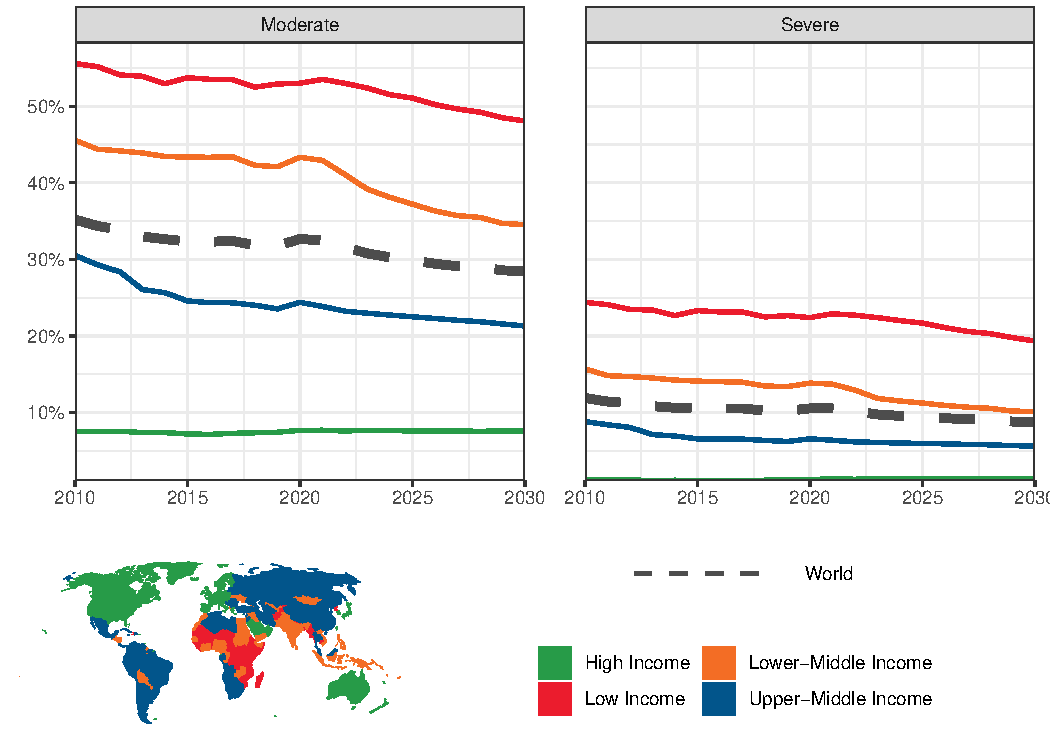
\includegraphics[width=\linewidth]{img/Rates.pdf}
  \caption{Percentage of the population over the threshold for moderate and severe food insecurity, by World Bank income groups as of 2020.}
  \label{fig:rates}
\end{figure}


\subsection{Food Insecurity Across Space}
We find substantial heterogeneity in the global distribution of severe food insecurity across countries and subnational regions (See Fig. \ref{fig:map}).  For the year 2020, mainland sub-Saharan Africa is the continent with the highest rates of severe food insecurity, with 20\% of people over the corresponding threshold in at least one subnational area in every country except Gabon, Djibouti and Equatorial Guinea.  Outside of Africa, serious pockets of severe food insecurity also occur in Venezuela, Syria, Papua New Guinea, Yemen, and Afghanistan.  In many large middle-income countries, severe food insecurity is also quite prevalent, with rates between 10\% and 15\% in northern Brazil, many central Asian and middle-eastern countries, as well as India and Indonesia.

The experience of at least moderate food insecurity is quite common in many parts of the world.  In 2020, much of Africa, south and southeast Asia, and parts of Latin America had over 50\% of the population living with moderate food insecurity.  Even in highly developed economies, such as the United States and parts of eastern and southern Europe, over 10\% of the population is above the threshold for moderate food insecurity.

\begin{landscape}
\begin{figure}[h]
  \centering
  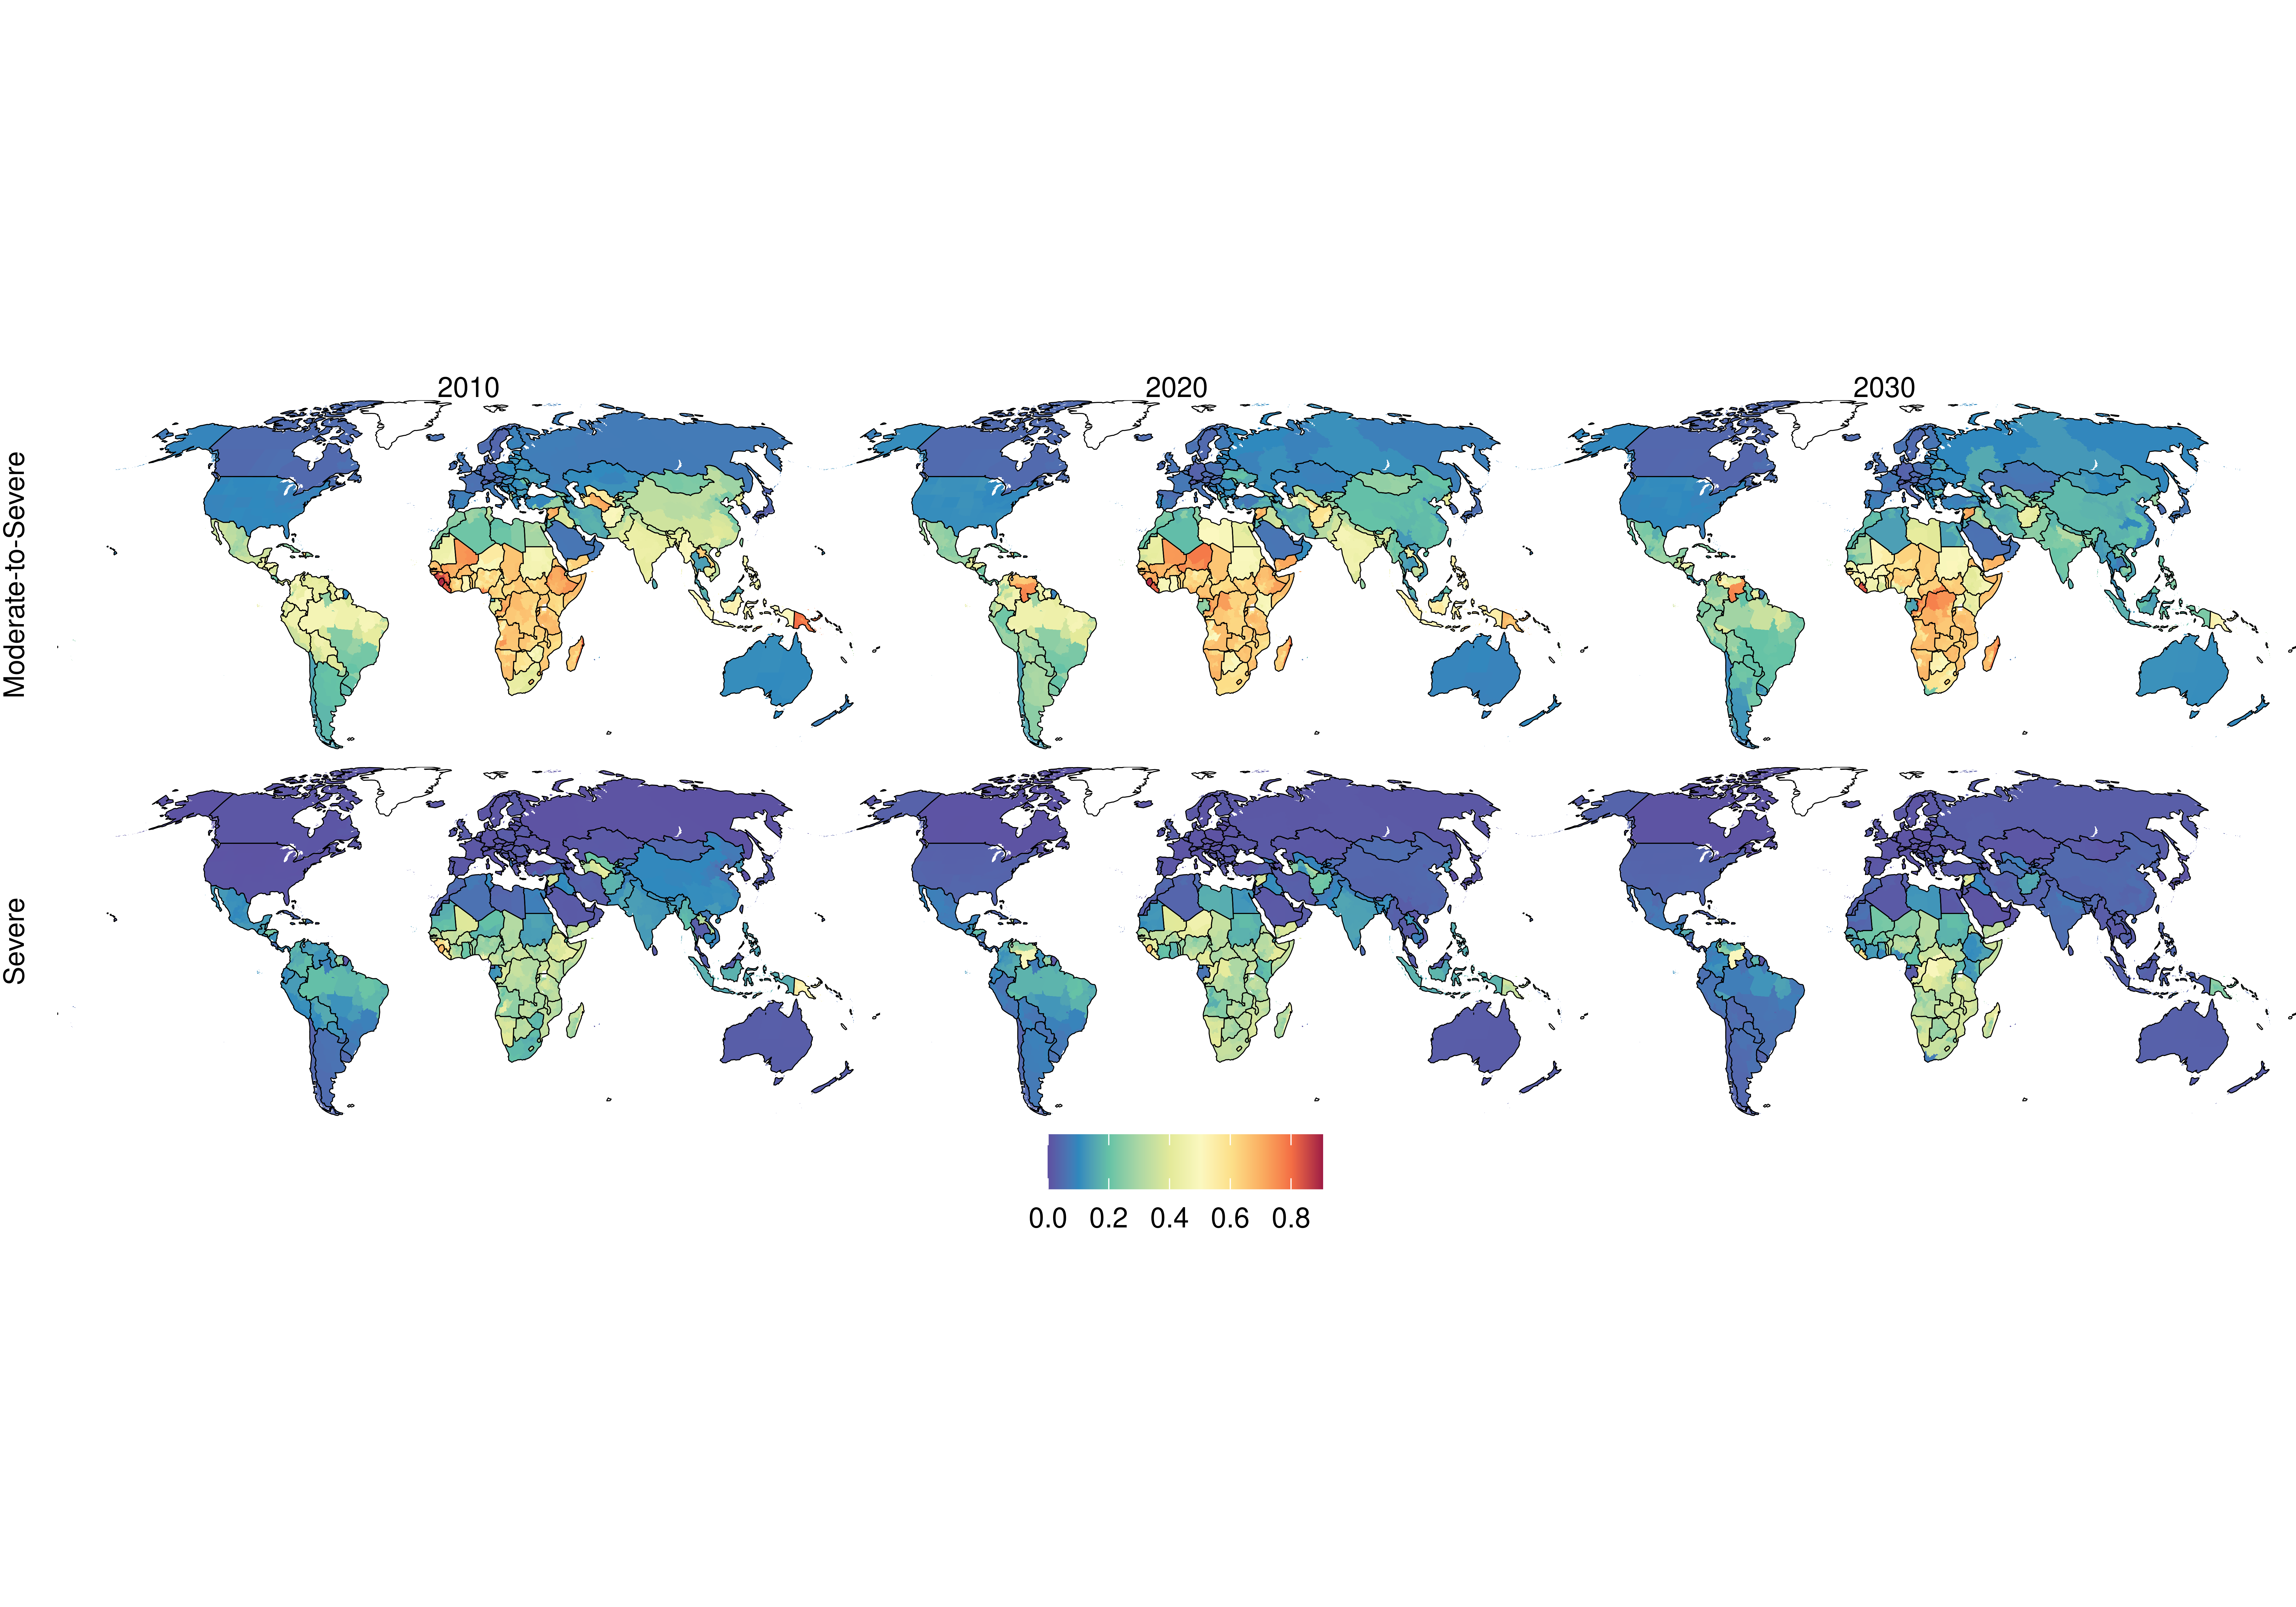
\includegraphics{img/FullMap.pdf}
  \caption{Spatial distribution of moderate and severe food insecurity for the years 2010, 2020, and 2030.}
  \label{fig:map}
\end{figure}
\end{landscape}

\subsection{Important Predictors of Food Insecurity}
Overall, our model was able to predict food insecurity with high accuracy in the countries for which training data was available ($R^2 = 0.950$ and $R^2 = 0.940$ for moderate and severe food insecurity, respectively), and excluding entire countries from the training data to evaluate out-of-country model error still showed overall good results ($R^2 = 0.792$ and $R^2 = 0.746$ for moderate and severe food insecurity, respectively).  The relative importance of different variables as predictors of food insecurity can be assessed by examining the loss in forecast accuracy resulting from the exclusion of particular covariates.

For severe food insecurity, the most important variable for predicting food security levels is the Poverty Headcount Index (See Fig. \ref{fig:vimp}, followed by the rate of stunting.  For predicting the rate of people with at least moderate food insecurity, GDP per capita is the most important, followed closely by the Poverty Headcount Index.  For the rate of severe food insecurity, the country's Gini coefficient was more important compared to moderate food insecurity.  Across both indicators, economic variables were the most relevant predictors.

\begin{figure}[h]
  \centering
  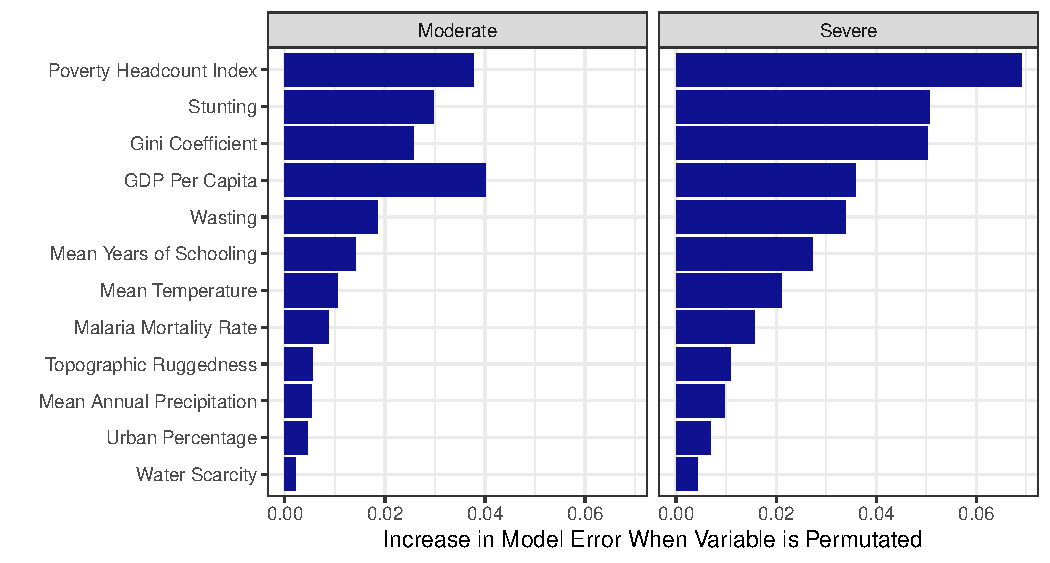
\includegraphics[width=\linewidth]{img/VIMP.pdf}
  \caption{Importance of each variable in predicting the percent of a population over thresholds for moderate and severe food insecurity.  This is determined by the increase in the error when the variable is permuted before fitting the model.}
  \label{fig:vimp}
\end{figure}

The results of this analysis can be further explored in more detail on the \href{https://worldhunger.io}{World Hunger Clock}, including statistics for each subnational administrative area.

\section{Discussion}
This paper presents the first global estimates of the experience of food insecurity at a subnational level, with forecasts until the year 2030.  We find that, while food insecurity has been increasing and has likely worsened in 2020 due to the economic downturn associated with the coronavirus pandemic, our models predict that the percent of people who experience food insecurity globally will decrease throughout the 2020s, largely because of progress in developing countries.  Nevertheless, lower and lower-middle income countries are expected to see overall increases in the number of food insecure people. 

Our analysis of the relative importance of different predictors for future food insecurity dynamics shows that economic conditions are the largest driver of global variation in rates of food insecurity. For both moderate and severe food insecurity, the Poverty Headcount Index, the Gini coefficient, and GDP per capita appear as highly relevant predictors of the rate of food insecurity. The rate of stunting, an indicator of both sanitary conditions and chronic, long-term under-nutrition is also an important predictor of food insecurity. However, other indicators of nutrition and sanitary conditions, such as the rates of wasting and malaria mortality are less important as explanatory factors of changes in food insecurity. Geographic and climate factors, such as the percentage of urban population, topographic ruggedness and mean annual temperature or precipitation do not appear to be robust predictors of food insecurity at a global scale. 

While economic conditions, and especially GDP per capita, are important predictors of food insecurity at a global scale, there is an upper limit to the extent to which increasing economic development alone can improve food security outcomes.  High income countries have seen little improvement in food insecurity outcomes over twenty years, and upper-middle income countries are expected to see diminishing gains throughout the 2020s.  Among the high-income countries in our dataset, those with the lowest rates of moderate and severe food insecurity also had lower inequality and poverty.  This suggests that our model's forecasted marginal increases in food insecurity in high income countries is due to trends of increasing income inequality, and that economic development alone cannot ensure that everyone is well-fed.

Our results anticipating increases in the number of people over the threshold for moderate food insecurity concur with the FAO's predictions of increased rates of undernourishment, the other indicator for the SDG 2 target of ending hunger \citep[Part 1, Page 11]{sofi2020}.  However, severe food insecurity may be a more apt indicator to compare with undernourishment, as the global totals are more similar \citep{sofi2020}.  In this case, our predictions diverge: the FAO estimates a 24\% increase, from 687 to 841 million undernourished people, from 2019 to 2030, whereas we predict a 2.6\% decrease, from 787 to 767 million severely food insecure people over the same period.

These discrepancies are in part due to our differing modeling approaches. While the SOFI report extrapolated recent trends in undernourishment and stunting, we modeled food insecurity based on interactions between projections in factors like GDP per capita, population, and the prevalence of stunting. Additionally, our diverging predictions for different hunger indicators are not necessarily mutually exclusive: it is theoretically possible for undernourishment to increase while severe food insecurity, as measured by the FIES, decreases.  The discrepancies between our projections and those of the FAO illustrate both the complexity of hunger as a social phenomenon, as well as the challenges in predicting future socioeconomic developments, where different modeling approaches may yield different forecasts.

When making predictions in countries where we do not have primary data, we assume that the relationships among variables like poverty, stunting, inequality, and hunger are the same across all locations.  We test the accuracy of these cases by using ten-fold cross validation at the country level, and we find good accuracy, with our models making estimates that are only off by 4-7 percentage points on average when applied to countries outside of the training set. 

Additionally, when making predictions into the future, we assume that the long-term patterns of demographic change, urbanization, and development will maintain their trajectories for the next decade.  At a global scale, this is almost certainly the case: it is highly unlikely that rates of fertility or economic growth will shift suddenly and globally.  Nevertheless, at more local scales, sudden crises can lead to severe and unforeseeable increases in food insecurity, as crises in the previous decade in Yemen, Syria and Venezuela have shown.

While we find that rates of food insecurity are expected to decrease overall by 2030, our model, which relies on middle-of-the-road assumptions, still expects the number of people experiencing moderate food insecurity to increase and the number of people experiencing severe food insecurity to fall only slightly between 2010 and 2030.  This still leaves billions of people eating less than they should and three-quarters of a billion people going entire days without eating a decade from now, a falling far short of the SDG 2 goal of ending hunger.  Moreover, decreases in food insecurity as measured by the FIES do not necessarily mean there will be improvements in other significant challenges such as poor dietary quality, micronutrient deficiencies, sustainable diets, or obesity.  Thus, while expected trends in correlates of food security give cause for optimism, there is still significant work to be done at the political level in pursuit of SDG 2.

\section{Methods}
\subsection{Disaggregation}
The data on the FIES collected by Gallup records many individual-level attributes from the respondents, including age, gender, wealth quintile, and whether they live in an urban or rural area.  Using national data on these variables, a standard weighting scheme is created for each individual, based on the ratio of population probabilities to sample probabilities of an individual with those characteristics being selected \citep{bethlehem2009applied}.  We use a similar methodology and calculate post-stratification weights at a subnational level.  We use year-specific subnational estimates of population shares by gender, age, urbanization, and, where available, wealth, and create a separate set of weights for each subnational area across all individuals.  For age and gender, we used gridded data from WorldPop \citep{Tatem2017}; for urbanization, we used spatially explicit estimates published by Jones and O'Neill \citep{Jones2016}; and for wealth we used data on household wealth quintiles from Demographic and Health Surveys \citep{dhsall}.  This methodology rests on the mild assumption that, within a given country, two individuals of the same age, gender, urbanization level and wealth quintile will have a similar food security status.

\subsection{Covariates}
We model subnational rates of moderate and severe food insecurity as a function of several covariates related to human development, nutrition, health, infrastructure, income levels and distribution, and the environment (See Table \ref{tab:covars}).  We employ covariates for which projections are available up to year 2030 and, in most cases, also have subnational spatial resolution.  For projections based on the Shared Socioeconomic Pathways (SSP) framework \citep{oneill2014new}, we use the middle-of-the-road pathway, SSP2, and for climatological variables, we use forecasts based on the Representative Concentration Pathway (RCP) 6.0 \citep{van2011representative}.  

Many of the variables require the harmonization of subnational historical data with projections at the national level.  These include mean years of schooling, GDP per capita, as well as population. We use observed trajectories in the historical distribution of variables among subnational areas within a country to predict the future distribution of GDP, population, and schooling among subnational areas and disaggregate national-level future projections.

For health variables that have historically shown long-term trends and represent a rate of occurrence in a population, including stunting, wasting, and malaria mortality rate, we estimate the Annualized Rate of Change (AROC) for each subnational area to model these and to obtain predictions up to variables for 2030. We calculate the rate of change between each pair of years in the dataset, and then use the mean rate of change over the period for which data are available, giving greater weight to more recent years, and applying that mean rate of change to estimate future levels.  This method is used to obtain forecasts of the rates of stunting and wasting up to the year 2030.

For the climatic variables, temperature and precipitation, we combine historical observations with an ensemble of four bias-corrected simulations of the future climate from the Inter-Sectoral Impact Model Intercomparison Project (ISIMIP) \citep{warszawski2014inter}.

Finally, we adjust several variables to account for the effects of the COVID-19 pandemic.  These include June 2020 GDP predictions from the World Bank \citep{prospects2020}, August 2020 estimates of impacts on anthropometry from \textit{The Lancet} \citep{headey2020impacts}, as well as the Poverty Headcount Index \cite{Cuaresma2018}.

\begin{table}[H]
  \centering
	\begin{tabular}{lll}
		\toprule
    Name & Source & Scale \\
		\midrule
    Urban Percentage & \citep{Jones2016} & Subnational \\
    Stunting & \citep{Local2020} & Subnational \\
    Wasting & \citep{Local2020} & Subnational \\
    Mean Years of Schooling & \citep{Smits2019, KC2017} & Subnational\\
    GDP Per Capita & \citep{Smits2019, Dellink2017} & Subnational \\
    Gini Coefficient & \citep{Rao2019a} & National\\
    Poverty Headcount Index & \citep{Cuaresma2018} & National \\
    Water Scarcity & \citep{greve2018global} & Subnational \\
    Mean Annual Precipitation &  \cite{abatzoglou2018terraclimate, warszawski2014inter} & Subnational \\
    Topographic Ruggedness &  \cite{USGS1996, Riley1999} & Subnational \\
    Mean Temperature &  \cite{abatzoglou2018terraclimate, warszawski2014inter} & Subnational \\
    Malaria (\textit{P. falciparum}) Mortality Rate &  \cite{Weiss2019} & Subnational \\
		\bottomrule
	\end{tabular}
	\caption{Covariates Included in the Analysis}
	\label{tab:covars}
\end{table}


\subsection{Modeling}
We fit two models for all subnational areas globally from 2010 to 2030: one for the percent of the population over the threshold for moderate food insecurity, and one for the percent of the population over the threshold for severe food insecurity.  We use random forest regressions, which perform well in the presence of non-linearities and interaction effects among predictor variables \citep{hastie2009elements}.  A random forest regression involves generating a large number of decision trees, each using different sub-samples of the data, and then aggregating the predictions of the decision trees.  By taking an ensemble of decision tree models, random forests introduce more variance and balance out the bias that is common to methods based on single decision trees \citep{friedman2001elements}. Given the bounded nature of our variables of interest, the random forest regression are applied to the logistically transformed rates.  We create our models using the \texttt{randomForestSRC} package in R \citep{ishwaran2019randomforestsrc}.

To get the best possible model performance, it is necessary to tune the hyperparamters, which control the process in which the random forest algorithm is run.  These include the average number of observations in a leaf node, the number of variables randomly selected as candidates for splitting a node, and the maximum depth of each tree.  We use the combination of hyperparameters that perform best under ten-fold cross validation based on $R^2$.

When performing cross validation, it is typical to select observations at random.  However, in our training data we have multiple highly similar observations from each country across years and subnational areas, and we extend our model predictions to countries that were not found at all in our training data.  Thus, we perform a type of leave-one-out cross validation, where we leave out all of the data from one country for each iteration.  Thus, the model error after cross validation gives us a sense of how the model is performing in countries where FIES data was not collected.  By this validation metric, we find that our models perform well, with an $R^2$ of 0.792 and mean average error (MAE) of 0.071 for moderate food insecurity and an $R^2$ of 0.746 and a MAE of 0.041 for severe food insecurity.  After fitting models on the entire dataset, we observe a within-sample $R^2$ of 0.950 and an MAE of 0.034 for moderate food insecurity and an $R^2$ of 0.945 and a MAE of 0.018 for severe food insecurity.

After fitting the models, we examine the importance of the individual covariates in explaining rates of moderate and severe food insecurity. We use a common method of permuting each individual variable and re-running the regressions, and then determining the difference in Mean Average Error (MAE) between the regression \citep{ishwaran2007variable, breiman2001random}.  This metric can provide some interpretability to model predictions.

The Supplementary Materials provide a detailed description of the data processing for the covariates, as well as implementation and validation of the random forest models.

\printbibliography

\end{document}
